% This is samplepaper.tex, a sample chapter demonstrating the
% LLNCS macro package for Springer Computer Science proceedings;
% Version 2.21 of 2022/01/12
%
\documentclass[runningheads]{llncs}
%
\usepackage[T1]{fontenc}
% T1 fonts will be used to generate the final print and online PDFs,
% so please use T1 fonts in your manuscript whenever possible.
% Other font encondings may result in incorrect characters.
%
\usepackage{graphicx}
\usepackage{gensymb}
\usepackage{hyperref}
\hypersetup{
    colorlinks=true,
    linkcolor=blue,
    filecolor=blue,
    citecolor = blue,
    urlcolor=cyan,
    }
%
% add package to add email icon next to the author name
\usepackage[misc,geometry]{ifsym}
%
% add package to use interactive orcid links next to author name
\usepackage{orcidlink}
%
% table things
\usepackage{array}
\newcolumntype{L}[1]{>{\raggedright\arraybackslash}p{#1}}
\newcolumntype{C}[1]{>{\centering\arraybackslash}p{#1}}
\newcolumntype{R}[1]{>{\raggedleft\arraybackslash}p{#1}}
\usepackage{float}
% Used for displaying a sample figure. If possible, figure files should
% be included in EPS format.
%
% If you use the hyperref package, please uncomment the following two lines
% to display URLs in blue roman font according to Springer's eBook style:
%\usepackage{color}
%\renewcommand\UrlFont{\color{blue}\rmfamily}
%
\begin{document}
%
\title{Automatic Whole Body FDG PET/CT Lesion Segmentation using Residual UNet and Adaptive Ensemble}
%
%\titlerunning{Abbreviated paper title}
% If the paper title is too long for the running head, you can set
% an abbreviated paper title here
%
\author{Gowtham Krishnan Murugesan\inst{1}\orcidlink{0000-0002-2160-6648} \and
    Diana McCrumb\inst{1}\orcidlink{0000-0001-7147-974X} \and
    Eric Brunner\inst{1}\and
    Jithendra Kumar\inst{1}\orcidlink{0000-0001-8714-5381} \and
    Jaya Khushalani\inst{1} \and
    Rahul Soni\inst{1} \and
    Vasily Grigorash\inst{1} \and
    Anthony Chang\inst{1} \and
    Anderson Peck\inst{1} \and
    Jeff VanOss\inst{1}\textsuperscript{(\Letter)}\orcidlink{0000-0002-0632-3519} \and
    Stephen Moore\inst{1}}

%
\authorrunning{G. Murugesan et al.}
% First names are abbreviated in the running head.
% If there are more than two authors, 'et al.' is used.
%
\institute{BAMF Health, Grand Rapids, Michigan 49503, USA\\
    \email{jeff.vanoss@bamfhealth.com}\\
}
%
\maketitle              % typeset the header of the contribution
%
\begin{abstract}
    Multimodal Positron Emission Tomography / Computed Tomography (PET/CT) plays a key role in malignant tumor diagnosis, staging, restaging, treatment response assessment and radiotherapy planning. The complementary nature between high resolution anatomic CT and high sensitivity/ specificity molecular PET imaging provides accurate assessment of disease status\cite{zaidi2008clinical}. In oncology, 18-fluorodeoxyglucose (FDG) PET/CT is the most widely used to identify and analyze metabolically active tumors.  In particular, FDG uptake allows more accurate detection of both nodal and distant forms of metastatic disease Accurate quantification and staging of tumors is the most important prognostic factor for predicting the survival of patients and to design personalized patient management plans \cite{kinahan2009pet}\cite{dirks2022computer}. Analyzing PET/CT quantitatively by experienced medical imaging experts/ radiologists is time consuming and error prone. Automated quantitative analysis by deep learning algorithms to segment tumor lesions will enable accurate feature extraction, tumor staging, radiotherapy panning and treatment response assessment. AutoPET challenge 2022 provided an open-source platform to develop and benchmark deep learning models for automated pet lesion segmentation by providing large open-source whole body FDG-PET/CT data. We trained fivefold cross validation on residual UNET’s to automatically segment lesions using multimodal PET/CT data from xxx subjects provided by autoPET MICCAI 2022 challenge and used adaptive ensemble highly contributive models output as final segmentation. We achieved xxx dice, xxx hausdroff, xxx sensitivity and xxx specificity in held out test data set (N=156).


    \keywords{CT  \and Abdominal organ segmentation \and Multiple organs \and nnUNet.}
\end{abstract}
%
%
%
\section{Introduction}
Whole body Positron emission tomography/computed tomography (PET/CT) is widely used modality in tumor imaging to evaluate the localized tumor burden, to detect symptomatic metastatic lesions early. PET/CT is a non-invasive means to quantify metabolically active tumors and plays a crucial role in initial diagnosis, staging, restaging, treatment planning and recurrence surveillance in a variety of cancers. Recent study shows that PET/CT can also provide early information on tumor response to therapy, potentially enabling personalized patient management \cite{ben200918f}.

Many PET based radiotracers are widely used in different malignant tumors. 18-fluorodeoxyglucose (18F-FDG) is the most commonly used radiotracers for oncologic imaging and is based on the increased glucose metabolism in malignant tumors \cite{shen2021evolving}\cite{jadvar2015positron}.  The conventional tracer 18F-FDG was efficient for detecting lesions that maintained high glucose metabolism both in the primary tumor and metastases. In solid tumors, 18F-FDG showed its high sensitivity for detecting metastases \cite{evangelista2020re}.

Annotation of lesions are done usually by expert radiologist to perform quantitative analysis. Automatic annotation of lesions is in need of an hour to avoid manual annotation of tumor is very labor-intensive, error prone and time-consuming, especially in whole-body FDG-PET scans.  Poor resolution and high statistical noise in PET images, uptake of FDG in several highly metabolic but normal, healthy tissues (e.g., brain and heart) in addition to tumor regions and a time-dependent blood pool signal, inter subject uptake variability, sparse tumor regions in whole body PET/CT, data acquisition variability poses further challenges in developing automatic algorithms for tumor segmentation \cite{jemaa2020tumor} \cite{arabi2021promise}. Recent developments in deep learning models achieving highly accurate PET/CT lesion segmentation in specific regions provides promising premise to address this issue.  A number of recent studies explored the potential of DL-based automated tumor segmentation from PET or hybrid PET/CT examinations. Several studies have been conducted focusing on single disease type or organs such as head and neck cancer, liver, lung and bone lesion \cite{xue2021multi},\cite{moreau2020deep},\cite{protonotarios2022few},\cite{murugesan2021head}.


Recent developments in deep learning models achieving highly accurate PET/CT lesion segmentation in specific regions provides promising premise to address this issue.  Several recent studies explored the potential of DL-based automated tumor segmentation from PET or hybrid PET/CT examinations. Several studies have been conducted focusing on single disease type or organs such as head and neck cancer, liver, lung and bone lesion. To extend the state of the art to segment whole body pet lesions, AutoPET challenge 2022 provided an open-source platform to develop and benchmark deep learning models for automated pet lesion segmentation by providing large open-source whole body FDG-PET/CT data. We trained a 3D residual UNET using five fold cross validation on AutoPET data and performed adaptive ensemble to get final results. Our method achieved top performing results in the challenge.

\begin{figure}
    \centering
    \includegraphics[width=\textwidth]{Fig.1.png}
    \caption{Representative Whole Body FDG PET/CT scans provided by AutoPET challenge with annotations} \label{fig1}
\end{figure}


\section{Materials and Methods}
\subsection{Data and Preprocessing}
Whole body FDG-PET/CT from 900 patients, including 1014 studies provided by autoPET challenge 2022 are used to train the models. Held out datasets consisting of 200 studies 100 studies originating from the same hospital as the training database and 100 are drawn from a different hospital with similar acquisition protocol is used to assess algorithm robustness and generalizability. In the preprocessing step, CT data is resamples to PET resolution and normalized. Two experts annotated training and test data: At the University Hospital Tübingen, a Radiologist with 10 years of experience in Hybrid Imaging and experience in machine learning research annotated all data. At the University Hospital of the LMU in Munich, a Radiologist with 5 years of of experience in Hybrid Imaging and experience in machine learning research annotated all data. The residual UNET model is trained on five fold crossvalidation using training set and uploaded into the challenge portal for testing in docker format.

\begin{figure}
    \centering
    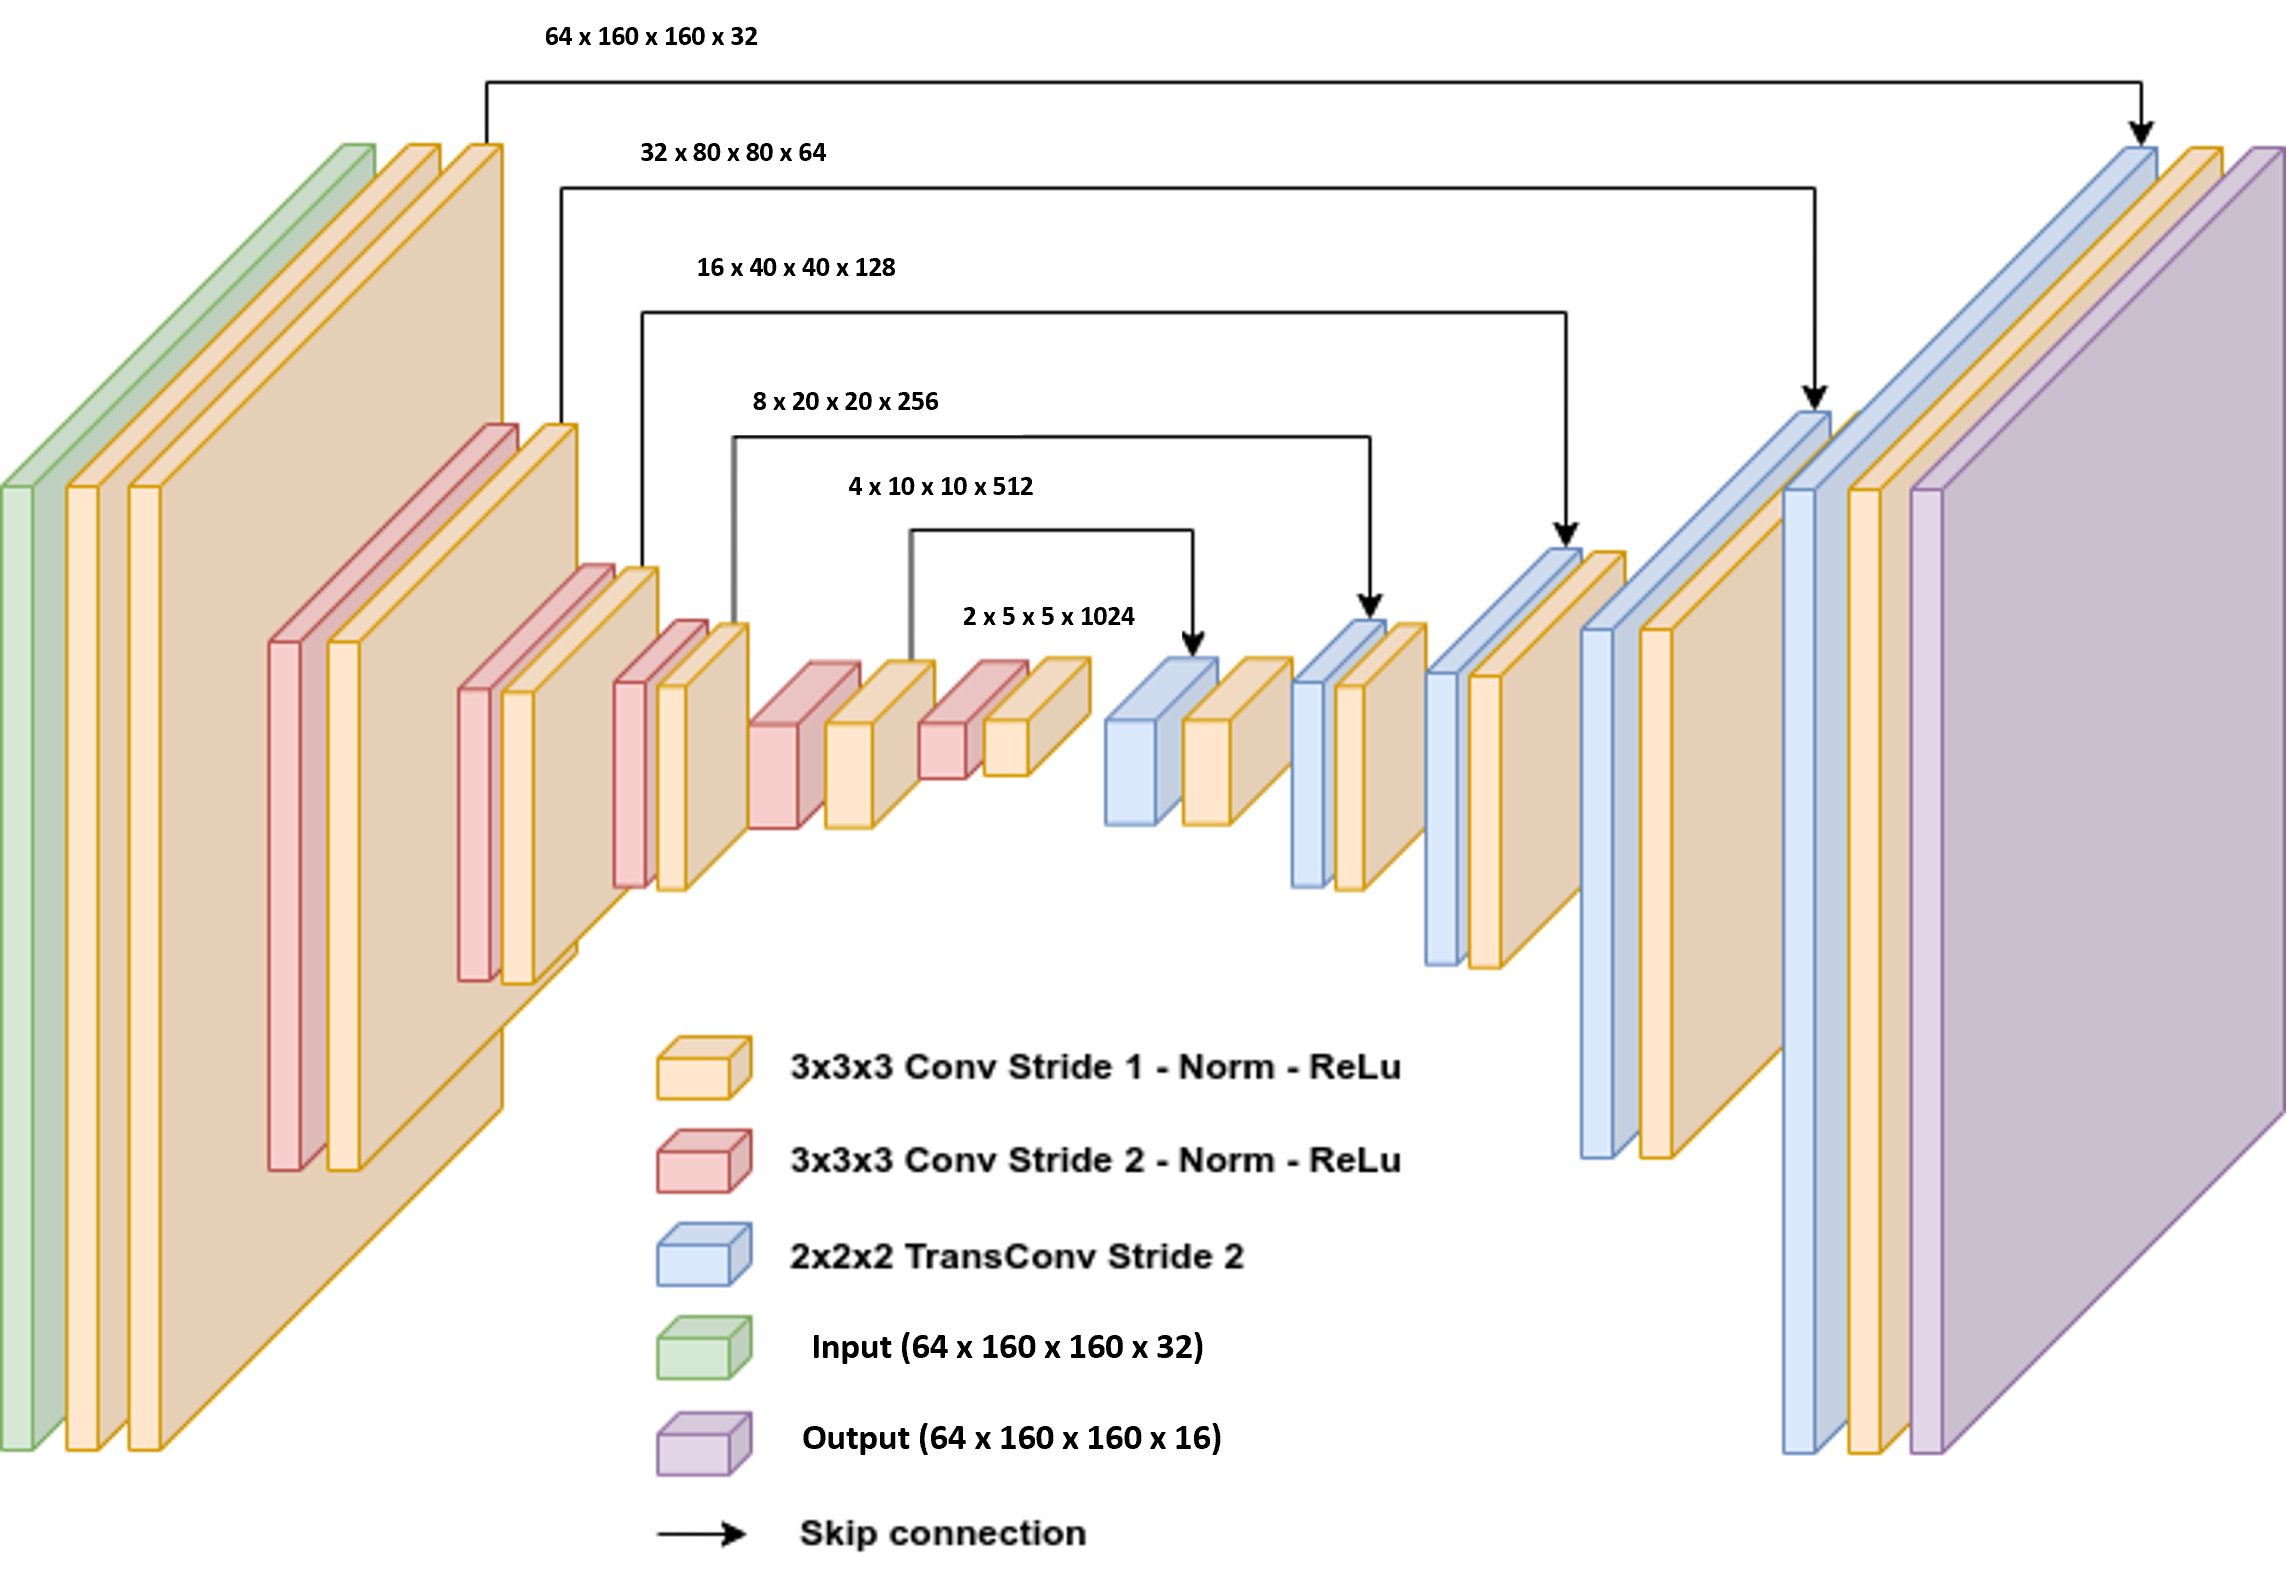
\includegraphics[width=\textwidth]{amos_model_architecture.png}
    \caption{The layers of the UNET architecture used. The input is a volume of 64x160x160 with one channels, CT. Input is resampled down five times by convolution blocks with strides of 2. On the decoder side, skip connections are used to concatenate the corresponding encoder layers to preserve spatial information.} \label{fig2}
\end{figure}
\begin{figure}
    \centering
    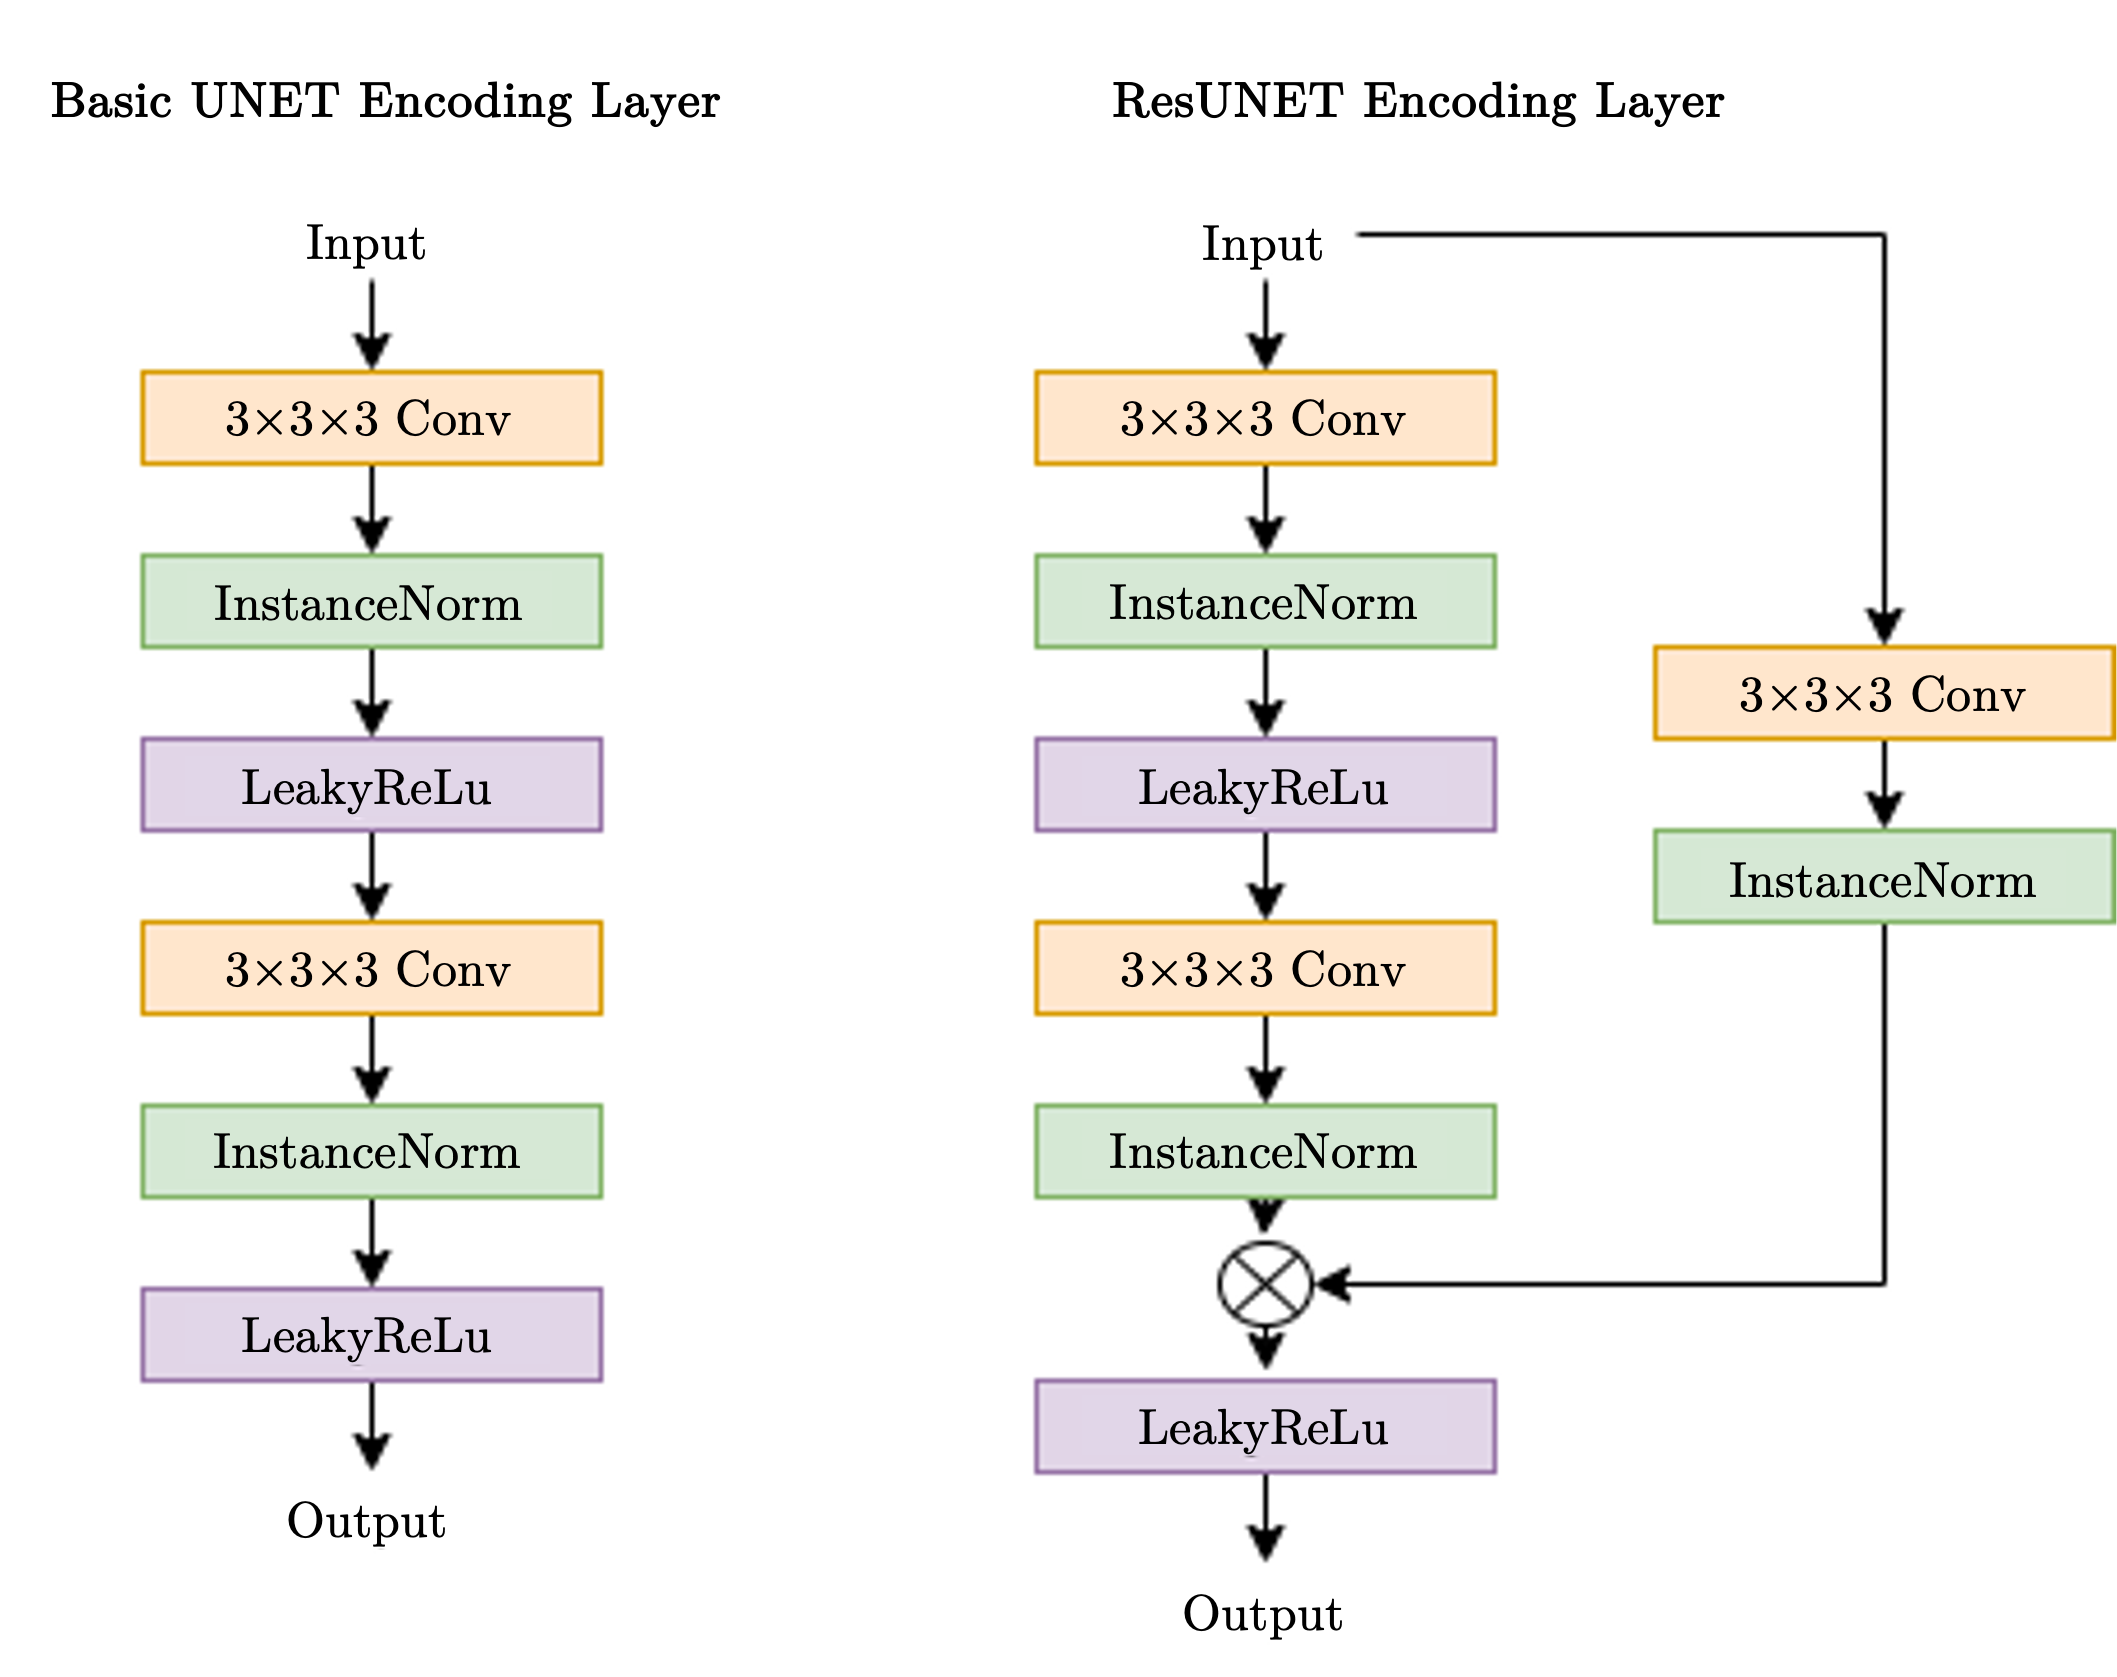
\includegraphics[width=80mm]{encoding-layer.png}
    \caption{In one instance of our UNET models, each encoding layer is a series of Convolution, normalization, and activation function repeated twice. In another instance, ResUNET, each encoding layer adds a residual path with convolution and normalization.} \label{fig3}
\end{figure}

\subsection{Model Training Methodology}
\subsubsection{Model Architecture} The nnUNET pipeline has achieved top tier performance in multiple medical imaging segmentation competitions. Analysis of the nnUNET pipeline and model architecture has shown that different variations sometimes perform better than the baseline nnUNET architecture \cite{murugesan2021head} \cite{Isensee}. From this, a standard a variant model using residual connections was proposed for training (see Fig. 2 and 3). The input image size of 64x160x160 with one channel, CT is used as input. Input is resampled down five times by convolution blocks with strides of 2. On the decoder side, skip connections are used to concatenate the corresponding encoder layers to preserve spatial information. Instance normalization and leaky ReLU activation in the network layers was used. This architecture initially used 32 feature maps, which then doubled for each down sampling operation in the encoder (up to 1024 feature maps) and then halved for each transposed convolution in the de-coder. The end of the decoder has the same spatial size as the input, followed by a 1x1x1 convolution into 1 channel and a SoftMax function. Models are trained for five folds with loss function of Dice Sorensen Coefficient (DSC) in combination with weighted cross entropy loss were trained.  To prevent overfitting augmentation techniques such as random rotations, random scaling, random elastic deformations, gamma correction augmentation, mirroring and elastic de-formation, were adopted. Each of the five models were trained for 1000 epochs with batch size of eight using SGD optimizer and learning rate of 0.01. Dice Similarity Coefficient (DSC), and normalized surface dice (NSD), will be used to assess different aspects of the performance of the segmentation methods.
% \begin{figure}
%     \centering
%     \includegraphics[width=80mm]{Figure 2. AMOS Predicted data.png}
%     \caption{Prediciton on three CT and three MRI scans from held out test scans using our method} \label{fig4}
% \end{figure}
% \begin{table}
%     \caption{Result on Task 1 (Only CT) and Task 2 (CT and MRI)}
%     \centering
%     \begin{tabular}{|l|l|l|l|l|}
%         \hline
%         \bfseries{Organ}               & \multicolumn{2}{c}{\bfseries{Dice}} & \multicolumn{2}{c}{\bfseries{NSD}}                                                                \\
%         \hline
%                                        & \bfseries{Task 1 (Only CT)}         & \bfseries{Task 2 (CT and MRI)}     & \bfseries{Task 1 (Only CT)} & \bfseries{Task 2 (CT and MRI)} \\
%         \hline
%         \bfseries{Spleen}              & 0.9701                              & 0.9712                             & 0.9125                      & 0.9157                         \\
%         \hline
%         \bfseries{Left Kidney}         & 0.9658                              & 0.9666                             & 0.9100                      & 0.9120                         \\
%         \hline
%         \bfseries{Right Kidney}        & 0.9656                              & 0.9664                             & 0.9060                      & 0.9083                         \\
%         \hline
%         \bfseries{Gallbladder}         & 0.8348                              & 0.8295                             & 0.7582                      & 0.7537                         \\
%         \hline
%         \bfseries{Esophagus}           & 0.8637                              & 0.8574                             & 0.7903                      & 0.7930                         \\
%         \hline
%         \bfseries{Liver}               & 0.9753                              & 0.9761                             & 0.8543                      & 0.8591                         \\
%         \hline
%         \bfseries{Stomach}             & 0.9302                              & 0.9299                             & 0.7957                      & 0.7925                         \\
%         \hline
%         \bfseries{Aorta}               & 0.9566                              & 0.9553                             & 0.9116                      & 0.9147                         \\
%         \hline
%         \bfseries{Postcava}            & 0.9219                              & 0.9217                             & 0.8093                      & 0.8183                         \\
%         \hline
%         \bfseries{Pancreas}            & 0.8840                              & 0.8863                             & 0.7505                      & 0.7556                         \\
%         \hline
%         \bfseries{Right Adrenal Gland} & 0.8055                              & 0.7869                             & 0.8398                      & 0.8312                         \\
%         \hline
%         \bfseries{Left Adrenal Gland}  & 0.8163                              & 0.8062                             & 0.8346                      & 0.8300                         \\
%         \hline
%         \bfseries{Duodenum}            & 0.8427                              & 0.8295                             & 0.7167                      & 0.7048                         \\
%         \hline
%         \bfseries{Bladder}             & 0.8997                              & 0.8907                             & 0.7830                      & 0.7752                         \\
%         \hline
%         \bfseries{Prostate/Uterus}     & 0.8512                              & 0.8427                             & 0.6564                      & 0.6498                         \\
%         \hline
%         \bfseries{Mean}                & \bfseries{0.8990}                   & \bfseries{0.8948}                  & \bfseries{0.8155}           & \bfseries{0.8169}              \\
%         \hline
%     \end{tabular}
% \end{table}
\subsection{Results}
We trained a five fold residual UNet model for automatic whole body lesion segmentation with robust mean dice of 0.8054 and 0.xxxx dice in validation and held out testing respectively.

\subsection{Discussion}
Our method achieved similar performance in both cross fold validationa dn unseen heldo out data showing that it generalized well multicenter data. Adaptive ensemble increased the performance by selectively picking model outputs with high contribution to final ensemble. \cite{murugesan2021head} and uncertainty aware segmentation correction may improve the segmentation performance.

\subsection{Conclusion}
We have trained a residual 3D UNet and achieved robust and generalized segmentation performance on automatic whole body FDG PET/CT lesion segmentation. We achieved xth rank in MICCAI AutoPET 2022 challenge out of xx teams participated.
% \clearpage
\bibliographystyle{splncs04}
\bibliography{AMOSbib}
\end{document}
